\section{Results and discussion}

\subsection{Scaling of the end to end distance}
\begin{Figure}
\centering
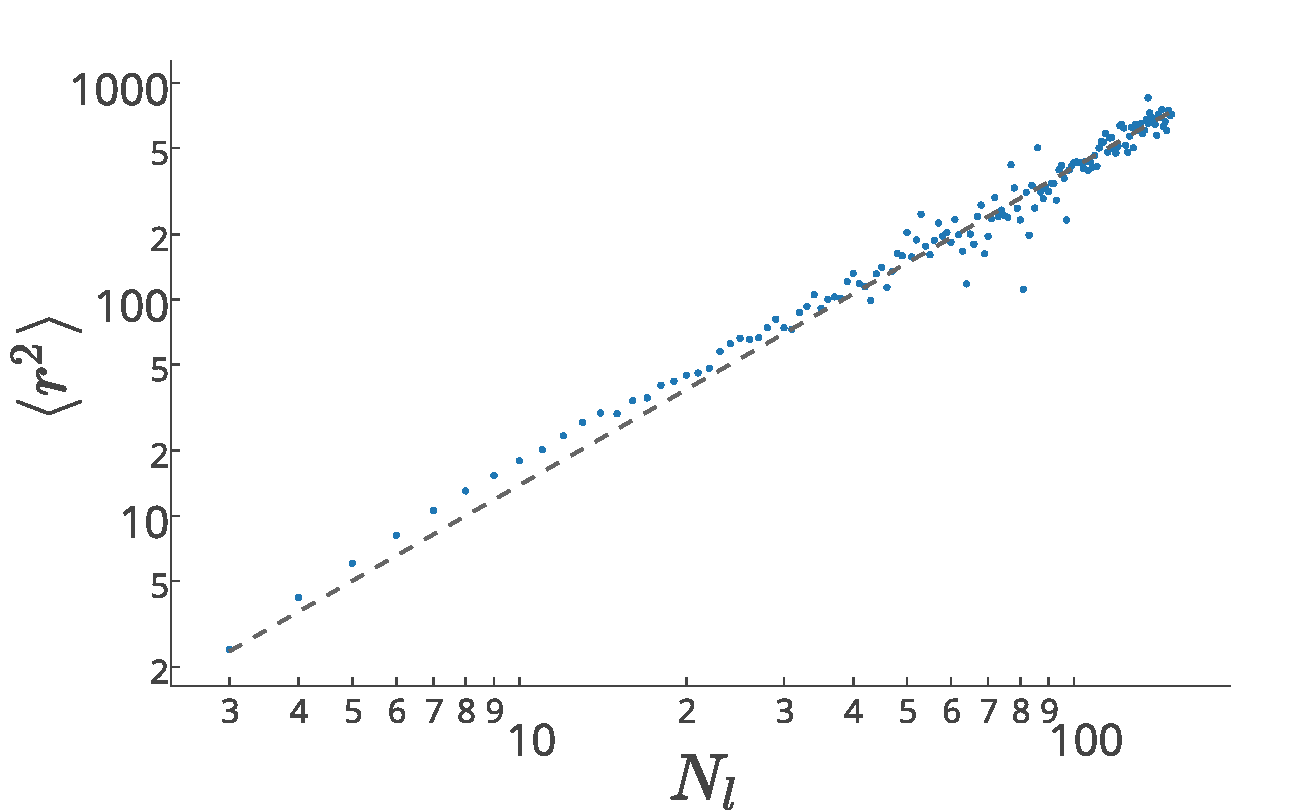
\includegraphics[width=\linewidth]{r_squared.pdf}
\captionof{figure}{Average end to end distance $\langle r^2\rangle$ as a function of polymer beads $N$ on a log scale. The blue dots depict $\langle r^2\rangle$ and the dashed line is fitted to $\langle r^2\rangle$ with $a\cdot N^{2\nu}$. The fitted value for $2\nu = 1.469 \pm 0.04246$.}
\label{fig:r_squared}
\end{Figure}

\subsection{Some notes on the program}
The energy calculations, LJ potential and bending energy, are for better performance written in Fortran. To make a connection between the Fortran code and the Python program, an interface is made using \emph{Fortran to Python interface generator} (F2PY). F2PY creates a Python C/API extension module that makes it possible to call the in Fortran written energy subroutine.

For low temperatures it is expected that the attractive part of the LJ-potential will dominate, causing the polymer to coil up. For higher temperatures, the repulsive part will always dominate, causing the polymer to expand. Since the LJ-potential is negligible beyond a distance of 2.5$\sigma$, the end to end distance will become independent on the temperature for high temperatures. Since a random walk will exhibit an end to end distance $r$ somewhere between these two regimes, it is expected that inbetween the two regimes the temperature $T_c$ can be found where $\langle r^2 \rangle$ equals $\langle r_{random}^2 \rangle$, where $\langle r_{random}^2 \rangle = N$ is the expectation value of the end to end distance squared for a random walk in 2 dimensions.
\begin{Figure}
  \centerfloat
     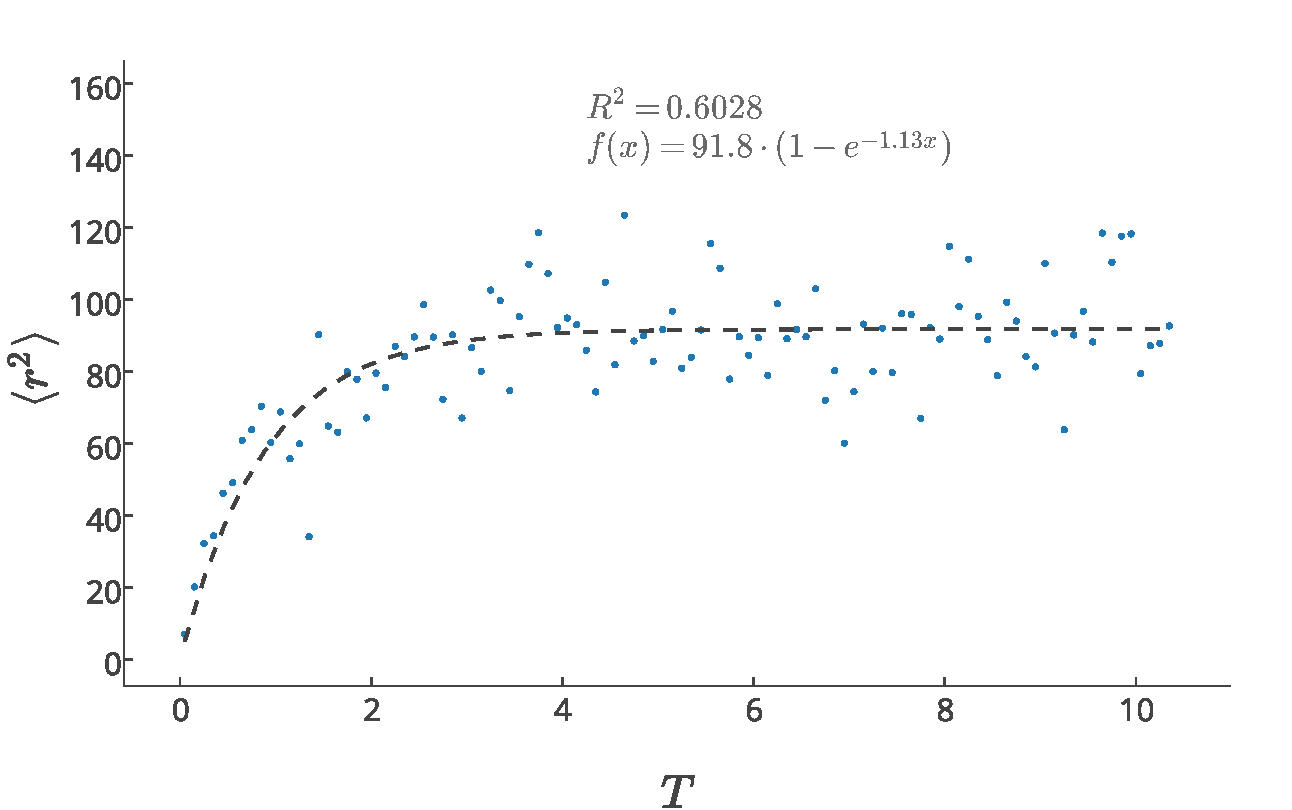
\includegraphics[scale=0.4]{end_to_end_distance_as_function_of_the_temperature.pdf}
 \captionof{figure}{Expectation value for the end to end distance squared as function of the temperature, for polymers with a length of 30 beads}\label{fig:end_to_end_afo_temperature}
\end{Figure}

Since for high temperatures $\langle r^2 \rangle$ becomes aprroximately constant, a fit function in the form of $a(1-e^{-bT})$ was chosen, with $a$ and $b$ the fit parameters. From the fit a value of $T_c \approx 0.35$ is found.
